\documentclass[AMA,Times1COL]{WileyNJDv5}

\articletype{Research Article}%

\received{Date Month Year}
\revised{Date Month Year}
\accepted{Date Month Year}
\journal{Statist.\ Med.}
\volume{00}
\copyyear{2025}
\startpage{1}

\raggedbottom

\usepackage{mathtools}
\usepackage{amssymb}
\newcommand{\hnABCD}{\mathrlap{\widehat{\phantom{\text{nA}}}}\text{nABCD}}

\graphicspath{{../figures/}}

\begin{document}

\title{Quantifying Effect Modifier Similarity for Regional Pooling in Multi-Regional Clinical Trials}

\author[1]{Author One}

\author[2]{Author Two}

\author[1]{Author Three}

\authormark{AUTHOR ONE \textsc{et al.}}
\titlemark{QUANTIFYING EFFECT MODIFIER SIMILARITY FOR REGIONAL POOLING}

\address[1]{\orgdiv{Department Name}, \orgname{Institution Name}, \orgaddress{\state{State}, \country{Country}}}

\address[2]{\orgdiv{Department Name}, \orgname{Institution Name}, \orgaddress{\state{State}, \country{Country}}}

\corres{Corresponding Author, Department Name, Institution Name, Address. \email{corresponding@institution.edu}}

\abstract[Abstract]{%
The ICH E17 guideline describes regional pooling in multi-regional clinical trials (MRCTs) in terms of the similarity of effect modifier distributions, but provides no quantitative methodology. We propose the normalized Area Between Cumulative Distributions (nABCD), a planning-stage dissimilarity index defined as the Wasserstein-1 distance divided by the pooled interquartile range. Unlike the standardized mean difference (SMD), nABCD captures differences in scale and skewness in addition to location---distributional features that may drive treatment effect heterogeneity through non-linear effect modification. Because nABCD requires only baseline effect modifier distributions, it can be computed from any representative data source, including prior trials, disease registries, and real-world evidence (RWE) databases---enabling a common planning scenario in which a small-sample region identifies suitable pooling partners before the trial begins. We develop a dual-pathway clinical calibration: when prior evidence on conditional average treatment effect (CATE) sensitivity ($L$) is available, nABCD is translated into a maximum potential regional treatment effect difference ($\Delta_{\max}$) with bootstrap confidence intervals; when $L$ is unknown, the framework reverse-calculates the required CATE sensitivity ($L^*$) at pre-specified clinical margins. Simulation studies across seven systematic scenarios demonstrated satisfactory bias and coverage of the percentile bootstrap estimator for non-negligible distributional differences at moderate sample sizes per region. We illustrate the framework through a hypothetical thrombolytic MRCT grounded in publicly available GUSTO-I individual patient data, with one region designated as a small-sample anchor and the remaining regions evaluated as pooling partners on two candidate effect modifiers (age and systolic blood pressure). Partner rankings differed markedly between the two effect modifiers, with several partners ranked similar on one but dissimilar on the other, demonstrating that all candidate effect modifiers must be evaluated jointly. A small subset of partners emerged as leading pooling candidates because they ranked low on both candidate effect modifiers and required clinically implausible CATE sensitivity to produce a meaningful treatment effect difference. The principal contribution of this work is to transform the previously qualitative judgment of ``similar enough'' into a reproducible quantitative basis for sponsor judgment, filling the methodological gap in ICH E17 implementation and supporting evidence-based regional pooling decisions from any representative population data source.}

\keywords{multi-regional clinical trial; ICH E17; effect modifier; Wasserstein distance; regional pooling; distributional similarity}

\jnlcitation{\cname{%
\author{Author One},
\author{Author Two}, and
\author{Author Three}}.
\ctitle{Quantifying effect modifier similarity for regional pooling in multi-regional clinical trials.} \cjournal{Statist.\ Med.} \cvol{2025;00:1--18}.}

\maketitle

\renewcommand\thefootnote{}
\footnotetext{\textbf{Abbreviations:} ABCD, area between cumulative distributions; AMI, acute myocardial infarction; CATE, conditional average treatment effect; CDF, cumulative distribution function; CI, confidence interval; EDF, empirical distribution function; EU, European Union; GUSTO, Global Utilization of Streptokinase and t-PA for Occluded coronary arteries; ICH, International Council for Harmonisation; IPD, individual patient data; IQR, interquartile range; KL, Kullback--Leibler; KS, Kolmogorov--Smirnov; MRCT, multi-regional clinical trial; nABCD, normalized area between cumulative distributions; NMPA, National Medical Products Administration; RWE, real-world evidence; SBP, systolic blood pressure; SMD, standardized mean difference; US, United States.}

\renewcommand\thefootnote{\fnsymbol{footnote}}
\setcounter{footnote}{1}

%==============================================================================
\section{Introduction}\label{sec:intro}
%==============================================================================

Multi-regional clinical trials (MRCTs), conducted across multiple countries or regulatory regions under a single protocol, have become the standard paradigm for global pharmaceutical development.\cite{chen2010,quan2010} This approach offers substantial benefits: accelerated timelines, broader generalizability, and earlier access to new therapies for patients worldwide. The International Council for Harmonisation (ICH) E17 guideline, adopted in 2017, established principles for planning and designing MRCTs, with a central assumption that treatment effects are generalizable across the target population.\cite{iche17}

Several regulatory authorities expect demonstration of treatment effect consistency in regional subpopulations,\cite{matsushima2024,song2025} yet individual regional sample sizes in global MRCTs are often insufficient for such demonstration. A key strategy for addressing this challenge is the \emph{regional pooling approach}, wherein regions with similar patient characteristics are grouped for analysis to enhance the ability to assess regional consistency.\cite{iche17} The ICH E17 guideline describes pooling decisions in terms of the similarity of effect modifier distributions.\cite{iche17}

An effect modifier is a baseline patient characteristic---such as age, disease severity, or genetic marker---for which the treatment benefit differs across subgroups. For example, if younger patients respond better to treatment than older patients, age is an effect modifier. When such heterogeneity exists, even if the drug works identically at the individual level, regions with different patient compositions may observe different average treatment effects. A region with predominantly younger patients would show larger benefits than a region with predominantly older patients, not because the drug works differently, but because the patient mix differs. This fundamental relationship underscores why effect modifier distributional similarity is critical to the validity of regional pooling. In this paper, we focus on continuous effect modifiers, such as age and disease severity scores; categorical effect modifiers raise distinct methodological considerations and are outside the present scope.

Despite the regulatory importance of effect modifier distributional similarity, current practice lacks a standardized quantitative methodology. The ICH E17 guideline provides no specific metric, threshold, or statistical procedure for determining when distributions are ``similar enough.'' Recent regulatory guidance has highlighted this gap. Song et al., writing from the China NMPA perspective on ICH E17 implementation, note the challenge of operationalizing pooling criteria without quantitative tools.\cite{song2025} Long et al.\ further discuss basic considerations for consistency evaluation under ICH E17.\cite{long2025}

This absence of quantitative tools is particularly acute at the \emph{planning stage}, when sponsors must identify suitable pooling partners for small-sample regions. The pooling rationale requires quantitative evidence that partner regions' patient populations are ``similar enough,'' yet no established method exists to provide such evidence. A workshop report by Matsushima et al.\ documented that regional imbalance in CRP-positive/MRI-negative status contributed to apparent inconsistency in the secukinumab MRCT.\cite{matsushima2024} This example illustrates the practical consequences when effect modifier distributional differences are not assessed quantitatively at the planning stage.

Although general-purpose comparison tools such as the standardized mean difference are routinely applied to baseline covariates,\cite{austin2011} they were not designed for assessing effect modifier distributional similarity across regions. As a single summary measure, the standardized mean difference cannot detect differences in variance or distributional shape. When effect modification is non-linear, these distributional features directly influence regional average treatment effects, and a comparison based on means alone will miss them.

This paper addresses these gaps by proposing the \emph{normalized Area Between Cumulative Distributions} (nABCD) as a quantitative index for assessing effect modifier distributional similarity across regions. nABCD is defined as the Wasserstein-1 distance between two cumulative distribution functions, normalized by a robust scale measure (the pooled interquartile range) to achieve scale-free interpretation. Unlike the standardized mean difference, nABCD captures differences in variance and shape simultaneously. We estimate nABCD with bootstrap confidence intervals and link it to clinical interpretation through a calibration framework. The Wasserstein distance provides a theoretically grounded measure of distributional dissimilarity in this setting.

The remainder of this paper is organized as follows. Section~\ref{sec:methods} presents the methodological framework, including the index definition, clinical calibration, and estimation procedure. Section~\ref{sec:simulation} describes a simulation study. Section~\ref{sec:application} demonstrates the framework using publicly available individual patient data. Section~\ref{sec:discussion} discusses implications, limitations, and future directions.

%==============================================================================
\section{Methods}\label{sec:methods}
%==============================================================================

An effect modifier is a factor for which the treatment effect varies across subgroups. Formally, let the conditional average treatment effect (CATE) be denoted $\tau(x) = E[Y(1) - Y(0) \mid X = x]$, where $X$ is the effect modifier. When this function is non-constant, the average treatment effect observed in region $r$ depends on the distribution $F_r$ of the effect modifier in that region:
\begin{equation}
\bar{\tau}_r = \int \tau(x) \, dF_r(x).
\label{eq:regional_ate}
\end{equation}
Assessing pooling suitability therefore requires a measure of distributional difference between regions.

\subsection{Existing Approaches and Their Limitations}\label{sec:existing}

The most widely used measure for comparing covariate distributions across groups is the standardized mean difference (SMD), defined as
\begin{equation}
\text{SMD} = \frac{\bar{X}_1 - \bar{X}_2}{S_{\text{pooled}}},
\label{eq:smd}
\end{equation}
where $\bar{X}_r$ denotes the sample mean in region $r$ and $S_{\text{pooled}}$ is the pooled standard deviation.\cite{austin2011} Because treatment effects in clinical trials are typically summarized as mean differences, SMD provides a scale-free comparison directly relevant to the quantities that drive clinical decision-making. However, by construction SMD captures only differences in location. Two distributions with identical means but markedly different variances---for example, $N(50, 5^2)$ and $N(50, 15^2)$---yield $\text{SMD} = 0$ despite a threefold difference in spread.

Distributional distance measures address this limitation by comparing distributions beyond summary statistics. Empirical distribution function (EDF) tests such as the Kolmogorov--Smirnov (KS) statistic, $D_{\text{KS}} = \sup_x |F_1(x) - F_2(x)|$, and related measures (Cram\'{e}r--von Mises, Anderson--Darling) quantify differences in the full shape of distributions by comparing CDFs directly. Information-theoretic divergences such as Kullback--Leibler (KL) divergence,
\begin{equation}
D_{\text{KL}}(P \| Q) = \int p(x) \log \frac{p(x)}{q(x)} \, dx,
\label{eq:kl}
\end{equation}
take a density-based approach, measuring how one probability distribution differs from another.

However, each of these approaches has limitations when applied to comparing effect modifier distributions across regions. SMD captures only location differences and is blind to variance and shape. EDF-based statistics such as the KS statistic capture full distributional differences but lack a clinically interpretable scale and have no theoretical connection to treatment effect heterogeneity. KL divergence is asymmetric---comparing region A to region B yields a different value than comparing B to A---can diverge to infinity when empirical distributions do not fully overlap, and requires density estimation that is impractical with small regional samples. Crucially, none of these measures offers a theoretical link that would translate a distributional distance into a bound on regional treatment effect differences. These gaps motivate a measure that (i) captures distributional features beyond location, (ii) provides a clinically interpretable scale, and (iii) offers such a theoretical link. The Wasserstein-1 distance and its clinical calibration, developed in the following subsections, satisfy all three requirements.

\subsection{Per-EM Wasserstein-1 Distance}\label{sec:nabcd_metric}

Among distributional distances that could capture the full distributional differences relevant to regional pooling, we adopt the Wasserstein-1 distance ($W_1$) for its unique theoretical connection to treatment effect heterogeneity (Proposition~\ref{prop:heterogeneity} below). The $W_1$ distance (sometimes called the Earth Mover's Distance) admits three equivalent representations on the real line, each highlighting a different facet of its interpretation.\cite{villani2009,vallender1974}

Let $F_1$ and $F_2$ denote the cumulative distribution functions (CDFs) of an effect modifier in two regions. Then
\begin{equation}
W_1(F_1, F_2) = \int_{-\infty}^{\infty} |F_1(x) - F_2(x)| \, dx = \int_0^1 |F_1^{-1}(u) - F_2^{-1}(u)| \, du = \inf_{\pi \in \Pi(F_1, F_2)} \int |x - y| \, d\pi(x, y),
\label{eq:wasserstein}
\end{equation}
where $F_r^{-1}$ is the quantile function and $\Pi(F_1, F_2)$ is the set of probability couplings with marginals $F_1$ and $F_2$. The CDF form expresses $W_1$ as the area between the two CDFs (Figure~\ref{fig:nabcd_definition}); the quantile form as the integrated absolute difference of quantile functions; and the Kantorovich form as the minimum expected absolute displacement to transport one distribution onto the other. The three forms are mathematically equivalent.\cite{vallender1974} Unlike the standardized mean difference, $W_1$ responds to differences in variance, skewness, and other distributional features.\cite{panaretos2019}

\begin{figure}[t]
\centerline{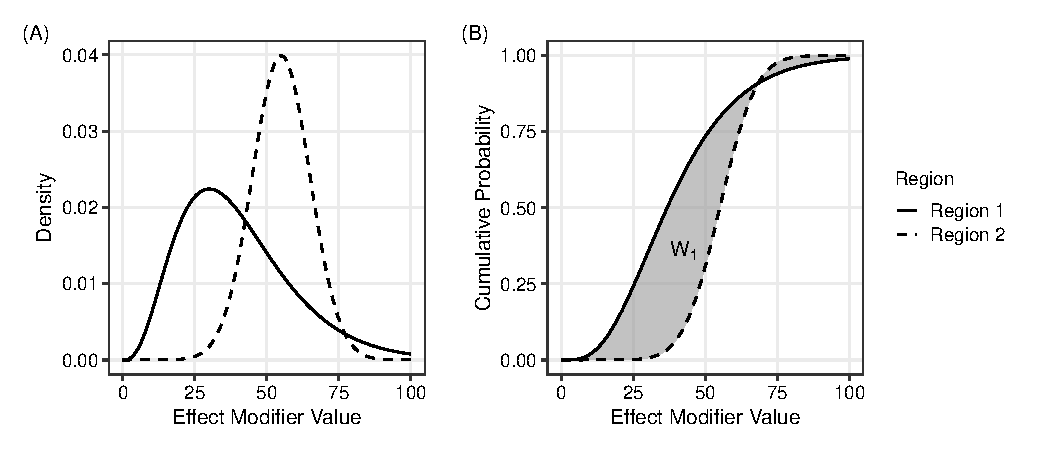
\includegraphics[width=0.8\textwidth]{fig1_w1_definition.pdf}}
\caption{The Wasserstein-1 distance as the area between cumulative distribution functions, illustrated with a right-skewed Region~1 (gamma distribution) and a symmetric Region~2 (normal distribution). Panel~(A): probability densities. Panel~(B): cumulative distribution functions; the shaded area equals $W_1(F_1, F_2)$.\label{fig:nabcd_definition}}
\end{figure}

A property of $W_1$ central to our framework is that it carries the units of the underlying effect modifier. In each of the three equivalent forms in equation~(\ref{eq:wasserstein}), the integrand has units of the variable $X$: the CDF values are dimensionless probabilities, the quantile function $F^{-1}$ returns values in the original measurement units, and the coupling integral sums distances $|x - y|$ in those units. Consequently, $W_1(F_1, F_2)$ is expressed on the original scale of the effect modifier. This dimensional alignment supports direct clinical interpretation: a regional $W_1 = 5$~mmHg in systolic blood pressure means that an expected 5~mmHg of probability mass must be transported between the two distributions to align them. The same logic precludes a meaningful direct comparison of $W_1$ values across effect modifiers measured on different scales, and we therefore restrict attention in this paper to per-effect-modifier assessment (Section~\ref{sec:discussion} elaborates on this scope choice).

$W_1$ is a proper metric on the space of probability distributions with finite first moment, satisfying non-negativity, symmetry, identity of indiscernibles, and the triangle inequality.\cite{villani2009} It is also affine-equivariant in the variable units, satisfying $W_1(F_{aX+b}, F_{aY+b}) = |a| \cdot W_1(F_X, F_Y)$ for any $a \neq 0$. Beyond these basic properties, $W_1$ admits a Kantorovich--Rubinstein dual representation\cite{villani2009}
\begin{equation}
W_1(F_1, F_2) = \sup_{\|f\|_{\text{Lip}} \leq 1} \left|\int f \, dF_1 - \int f \, dF_2\right|,
\label{eq:dual}
\end{equation}
which expresses $W_1$ as the largest possible difference in expected values of a 1-Lipschitz function $f$ between the two distributions (the notation $\|f\|_{\text{Lip}} \leq 1$ means $|f(x) - f(y)| \leq |x - y|$ for all $x, y$). If the conditional average treatment effect function $\tau(x)$ is Lipschitz continuous with constant $L_{\text{clinical}}$, so that $|\tau(x) - \tau(y)| \leq L_{\text{clinical}} |x - y|$ for all $x, y$, then $\tau / L_{\text{clinical}}$ is 1-Lipschitz and applying equation~(\ref{eq:dual}) yields the central result of this section:

\begin{proposition}\label{prop:heterogeneity}
\textup{(Connection to heterogeneity).} If the CATE function is Lipschitz continuous with constant $L_{\text{clinical}}$, then for any two regions with effect modifier distributions $F_1$ and $F_2$,
\begin{equation}
|\bar{\tau}_1 - \bar{\tau}_2| \leq L_{\text{clinical}} \cdot W_1(F_1, F_2).
\label{eq:heterogeneity_bound}
\end{equation}
\end{proposition}

\begin{proof}
Apply equation~(\ref{eq:dual}) with $f = \tau / L_{\text{clinical}}$, which is 1-Lipschitz by assumption. This yields $\left|\int (\tau / L_{\text{clinical}}) \, d(F_1 - F_2)\right| \leq W_1(F_1, F_2)$. Combining with equation~(\ref{eq:regional_ate}) for $\bar{\tau}_r$ and rearranging yields equation~(\ref{eq:heterogeneity_bound}).
\end{proof}

\noindent The bound in equation~(\ref{eq:heterogeneity_bound}) is specific to $W_1$. The $W_2$ distance, while admitting closed-form expressions for Gaussian families, does not possess a Lipschitz dual representation and therefore cannot provide an analogous bound. The alternative measures discussed in Section~\ref{sec:existing} similarly lack any analogous property.\cite{gibbs2002} Its right-hand side involves $W_1$ in its original measurement units, multiplied by a clinical slope $L_{\text{clinical}}$; no further normalization of $W_1$ is required to obtain a clinically interpretable bound. We therefore adopt $W_1$ in its original units as the primary similarity metric throughout this paper. Some prior literature has considered normalizing $W_1$ by a within-effect-modifier scale measure such as the pooled interquartile range; we show in Section~\ref{sec:inference} and Supplement~A that such normalization is mathematically redundant once equation~(\ref{eq:heterogeneity_bound}) is used for clinical calibration. The Lipschitz assumption underlying Proposition~\ref{prop:heterogeneity} is appropriate when the CATE function varies smoothly with the effect modifier; for threshold or step-function CATEs, $L_{\text{clinical}}$ can be arbitrarily large and the bound becomes conservative (Section~\ref{sec:discussion}).

\subsection{Estimation}\label{sec:estimation}

Given samples $\{X_{1,i}\}_{i=1}^{n_1}$ from region 1 and $\{X_{2,j}\}_{j=1}^{n_2}$ from region 2, the Wasserstein-1 distance is estimated using empirical distribution functions. Since $\hat{F}_1$ and $\hat{F}_2$ are piecewise constant (right-continuous step functions), the integral in equation~(\ref{eq:wasserstein}) reduces to a finite sum over the intervals defined by the combined order statistics:
\begin{equation}
\widehat{W}_1 = \sum_{k=1}^{n_1+n_2-1} |\hat{F}_1(x_{(k)}) - \hat{F}_2(x_{(k)})| \cdot (x_{(k+1)} - x_{(k)}),
\label{eq:estimator}
\end{equation}
where $\hat{F}_r$ denotes the empirical CDF (right-continuous) of region $r$ and $x_{(1)} < \cdots < x_{(n_1+n_2)}$ are the combined order statistics. The estimator $\widehat{W}_1$ inherits the original measurement units of the effect modifier. The asymptotic distribution of $W_1$ is non-standard: del Barrio et al.\cite{delbarrio1999} showed that $\sqrt{n}\,W_1(\hat{F}_n, F) \xrightarrow{d} \int |B(F(x))|\,dx$, where $B$ is a standard Brownian bridge. Because the quantiles of this limiting distribution depend on the unknown $F$, no universal critical values are available and direct construction of asymptotic confidence intervals is impractical. We therefore employ the nonparametric percentile bootstrap with $B = 2{,}000$ replicates.\cite{efron1993} In the two-sample setting, when $F_1 \neq F_2$ the Hadamard derivative of the $L_1$ functional is linear, so the ordinary nonparametric bootstrap is consistent.\cite{sommerfeld2018} Convergence occurs at rate $\sqrt{n_1 n_2/(n_1+n_2)}$ (see Appendix~\ref{app:asymptotic} for details). The estimator~(\ref{eq:estimator}) is computed in $O((n_1 + n_2) \log(n_1 + n_2))$ time, dominated by sorting the combined order statistics.

\subsection{Interpretation and Clinical Calibration}\label{sec:inference}

A central feature of $W_1$ is its connection to treatment effect heterogeneity through Proposition~\ref{prop:heterogeneity}. This connection provides the basis for a clinically grounded interpretation framework rather than reliance on fixed numerical cutoffs.

We refer to the Lipschitz constant of the CATE function $\tau(x)$ as the clinical slope $L_{\text{clinical}}$. By definition, $L_{\text{clinical}}$ quantifies the maximum change in the treatment effect per unit change in the effect modifier, expressed on the outcome scale of the trial---for example, percentage points of 30-day mortality per year of age, or percentage points per mmHg of systolic blood pressure. When $L_{\text{clinical}}$ is estimable from prior data, individual patient data (IPD) meta-regression on treatment-by-covariate interaction provides a per-unit slope directly,\cite{riley2010,fisher2017} and the same quantity is denoted the interaction slope in the methodological literature.\cite{vanderweele2014,vanderweele2019} More commonly at the MRCT planning stage, however, published subgroup reports document the direction and significance of interaction rather than a per-unit slope, and a precise numerical $L_{\text{clinical}}$ is unavailable. We address both situations below.

From Proposition~\ref{prop:heterogeneity}, the maximum potential difference in regional average treatment effects attributable to effect modifier distributional differences is
\begin{equation}
\Delta_{\max} = L_{\text{clinical}} \cdot W_1(F_1, F_2),
\label{eq:delta_max}
\end{equation}
expressed in the units of the trial outcome scale. The formula is invariant to within-effect-modifier scale normalization of $W_1$: as shown in Supplement~A, any normalized form $W_1 / X$ multiplied by the same scale $X$ cancels in equation~(\ref{eq:delta_max}), so adopting $W_1$ in its original units yields the same clinical-scale calibration as any rescaled version. When $L_{\text{clinical}}$ is independently known, equation~(\ref{eq:delta_max}) provides a direct clinical-scale translation of the observed distributional difference. When $L_{\text{clinical}}$ is unknown, the relation can be inverted to ask which $L_{\text{clinical}}$ would be required for a given $W_1$ to produce a clinically meaningful $\Delta_{\max}$.

The estimator $\widehat{W}_1$ has a percentile bootstrap CI (Section~\ref{sec:estimation}), and inferential uncertainty propagates linearly to $\Delta_{\max}$ when $L_{\text{clinical}}$ is treated as fixed: $[\Delta_{\max,L}, \Delta_{\max,U}] = L_{\text{clinical}} \cdot [W_{1,L}, W_{1,U}]$. When $L_{\text{clinical}}$ itself is uncertain or unavailable, we solve equation~(\ref{eq:delta_max}) for $L_{\text{clinical}}$ at a pre-specified clinical margin $\Delta_{\text{clin}}$ (the minimal clinically important treatment effect difference, the non-inferiority margin, or the targeted overall effect), yielding the required clinical slope
\begin{equation}
L^* = \frac{\Delta_{\text{clin}}}{W_1(F_1, F_2)}.
\label{eq:lstar}
\end{equation}
$L^*$ is the smallest clinical slope under which the observed distributional difference would produce a clinically meaningful regional treatment effect difference. If a plausible upper bound on $L_{\text{clinical}}$ from prior evidence (denoted $L_{\text{UB}}$) lies below $L^*$, the distributional difference is unlikely to translate into clinical heterogeneity, regardless of the unknown true $L_{\text{clinical}}$. The two pathways---forward calibration via equation~(\ref{eq:delta_max}) when $L_{\text{clinical}}$ is known and reverse comparison via equation~(\ref{eq:lstar}) against $L_{\text{UB}}$ when $L_{\text{clinical}}$ is unknown---accommodate the full range of evidence states encountered at the MRCT planning stage.

Specifying $L_{\text{clinical}}$ (or its upper bound $L_{\text{UB}}$) draws on disease-area evidence. For the GUSTO-I case study presented in Section~\ref{sec:application}, the Fibrinolytic Therapy Trialists' meta-analysis\cite{ftt1994} and GUSTO-I subgroup analyses\cite{gusto1993,lee1995} together support a conservative upper bound of $L_{\text{UB,age}} \approx 1 \times 10^{-2}$ per year and $L_{\text{UB,SBP}} \approx 2 \times 10^{-3}$ per mmHg on the 30-day mortality scale. ``Conservative'' here indicates that the chosen bounds exceed the empirical prognostic age slope of approximately $6 \times 10^{-3}$ per year reported by Lee et al.,\cite{lee1995} so that any plausible CATE sensitivity falls below them. Supplement~D discusses the derivation of these bounds, alternative specification strategies such as the deft estimator of Fisher et al.,\cite{fisher2017} and the limitations of class-level evidence. The methodology does not require an exact $L_{\text{clinical}}$; sensitivity analyses across a plausible range of values, or comparison of $L^*$ to $L_{\text{UB}}$, accommodate the typical uncertainty in this parameter.

The pooling assessment proceeds by computing per-effect-modifier $W_1$ with bootstrap CIs across candidate partner regions, deriving $\Delta_{\max}$ when $L_{\text{clinical}}$ is known or $L^*$ at a pre-specified $\Delta_{\text{clin}}$ when $L_{\text{clinical}}$ is unknown, and ranking partners by these quantities. The framework is deliberately estimation-centered rather than testing-based: $W_1$ has no universal cutoff that separates ``similar'' from ``dissimilar,'' and the appropriate threshold depends on the clinical slope $L_{\text{clinical}}$, which is external to the distributional comparison. By presenting per-pair $\Delta_{\max}$ (or $L^*$) with bootstrap CIs alongside the clinical context---the overall treatment effect size, the non-inferiority margin, the minimal clinically important difference---the framework provides quantitative inputs for sponsor and regulatory judgment without forcing a binary accept/reject decision.\cite{wasserstein2016}

%==============================================================================
\section{Simulation Study}\label{sec:simulation}
%==============================================================================

We conducted simulation studies to evaluate the estimation properties of the $\widehat{W}_1$ estimator: bias, variability, and coverage probability of bootstrap confidence intervals. These properties are essential for the clinical calibration framework, as reliable estimation of $W_1$ directly determines the quality of $\Delta_{\max}$ estimates via equation~(\ref{eq:delta_max}). Because the absolute scale of $W_1$ varies with the natural units of each distributional family considered, we present results throughout this section in the dimensionless ratio $\widehat{W}_1 / \widehat{\text{IQR}}_{\text{pooled}}$ for cross-scenario comparability; the corresponding bootstrap distribution of $\Delta_{\max}$ is invariant to this normalization choice (Supplement~A), so the operating characteristics displayed below carry directly to the clinical-scale quantities used in the methodology. We assessed performance across a range of scenarios relevant to MRCT applications.

\subsection{Simulation Design}\label{sec:sim_design}

\subsubsection{Scenarios}

We designed seven systematic scenarios for methodological validation, examining controlled distributional differences across location, scale, and combinations thereof. Table~\ref{tab:scenarios} summarizes these scenarios with their true values of $W_1 / \text{IQR}_{\text{pooled}}$, the dimensionless presentation form used throughout this section.

\begin{table}[ht]
\centering
\caption{Simulation scenarios with clinical motivations.\label{tab:scenarios}}
\begin{tabular}{lllll}
\toprule
\textbf{ID} & \textbf{Description} & \textbf{Distribution 1} & \textbf{Distribution 2} & \textbf{True $W_1 / \text{IQR}_{\text{pooled}}$} \\
\midrule
S1 & Null (identical) & $N(50, 10^2)$ & $N(50, 10^2)$ & 0.000 \\
S2 & Location 0.2$\sigma$ & $N(50, 10^2)$ & $N(52, 10^2)$ & 0.146 \\
S3 & Location 0.5$\sigma$ & $N(50, 10^2)$ & $N(55, 10^2)$ & 0.358 \\
S4 & Location 1.0$\sigma$ & $N(50, 10^2)$ & $N(60, 10^2)$ & 0.656 \\
S5 & Scale 1.5$\times$ & $N(50, 10^2)$ & $N(50, 15^2)$ & 0.244 \\
S6 & Skew (Log-normal) & $N(50, 10^2)$ & LogN$(\mu, \sigma)$ & 0.606 \\
S7 & Location + Scale & $N(50, 10^2)$ & $N(55, 15^2)$ & 0.347 \\
\bottomrule
\end{tabular}
\begin{tablenotes}
\item The Log-normal in S6 is parameterized to match mean 50 with CV $\approx$ 53\%, typical of clinical biomarkers such as ALT. S7 combines location and scale differences, representing the most realistic MRCT pattern. Tabulated values are computed via Monte Carlo integration ($n_{\textup{MC}} = 10^6$) using the population pooled IQR; operating characteristics of $\widehat{W}_1$ in any original measurement unit follow by multiplying tabulated entries by the corresponding $\text{IQR}_{\text{pooled}}$.
\end{tablenotes}
\end{table}

\subsubsection{Simulation Parameters}

For each scenario, we generated samples of size $n = 50$, 100, and 200 per region, reflecting sample sizes typical in MRCT regional subgroups. We performed 10{,}000 replications per scenario--sample size combination to ensure stable estimates of operating characteristics, with Monte Carlo standard errors below 0.005 for all reported proportions. Bootstrap confidence intervals were computed using $B = 2{,}000$ resamples. All simulations were conducted in R version 4.5.1.

\subsubsection{Evaluation Metrics}

Consistent with the estimation-centered framework, and writing $\hat{\rho} = \widehat{W}_1 / \widehat{\text{IQR}}_{\text{pooled}}$ and $\rho = W_1 / \text{IQR}_{\text{pooled}}$ for the dimensionless ratio, we evaluated:
\begin{enumerate}[1.]
\item Bias: $\text{Mean}(\hat{\rho}) - \rho$
\item Root mean squared error (RMSE): $\sqrt{\text{Mean}[(\hat{\rho} - \rho)^2]}$
\item Coverage probability: Proportion of 95\% bootstrap CIs containing the true value
\item CI width: Mean width of bootstrap CIs, reflecting estimation precision
\end{enumerate}

\subsection{Results}\label{sec:sim_results}

\subsubsection{Point Estimation and Coverage}

Table~\ref{tab:bias} presents the bias of $\hat{\rho}$ across scenarios and sample sizes. The estimator showed positive bias under the null hypothesis (S1), with bias decreasing from 0.185 at $n=50$ to 0.094 at $n=200$. This positive bias arises because the non-negativity of $W_1$ yields $\widehat{W}_1 > 0$ (and hence $\hat{\rho} > 0$) with probability 1 in finite samples, even when the true value equals zero ($F_1 = F_2$ almost everywhere). The estimator remains consistent ($\hat{\rho} \to 0$ as $n \to \infty$), but the convergence is slow near the parameter space boundary.

\begin{table}[ht]
\centering
\caption{Bias of $\hat{\rho}$ by scenario and sample size.\label{tab:bias}}
\begin{tabular}{lcccc}
\toprule
\textbf{Scenario} & \textbf{True $\rho$} & $\boldsymbol{n=50}$ & $\boldsymbol{n=100}$ & $\boldsymbol{n=200}$ \\
\midrule
S1 (Null) & 0.000 & 0.185 & 0.132 & 0.094 \\
S2 (0.2$\sigma$) & 0.146 & 0.078 & 0.038 & 0.017 \\
S3 (0.5$\sigma$) & 0.358 & 0.023 & 0.009 & 0.005 \\
S4 (1.0$\sigma$) & 0.656 & 0.014 & 0.006 & 0.003 \\
S5 (Scale) & 0.244 & 0.056 & 0.028 & 0.014 \\
S6 (Skew) & 0.606 & 0.034 & 0.016 & 0.010 \\
S7 (Loc+Scale) & 0.347 & 0.049 & 0.027 & 0.015 \\
\bottomrule
\end{tabular}
\begin{tablenotes}
\item Bias is defined as $\text{Mean}(\hat{\rho}) - \rho$, where $\rho = W_1 / \text{IQR}_{\text{pooled}}$. Results based on 10{,}000 replications with $B = 2{,}000$ bootstrap resamples.
\end{tablenotes}
\end{table}

For scenarios with true $\rho$ above approximately 0.2, bias was less than 0.04 in absolute value at $n \geq 100$, indicating satisfactory point estimation performance at practical sample sizes (Figure~\ref{fig:simulation}(A)). For S4 (1.0$\sigma$ location shift), bias was negligible (0.014 at $n=50$, 0.003 at $n=200$), confirming accurate estimation even for large distributional differences. For scenarios near the boundary (S1, S2), positive bias was more pronounced and diminished slowly with sample size---a well-known phenomenon for non-negative statistics where sampling variability inflates estimates when the true value is close to zero.

\begin{figure*}[t]
\centerline{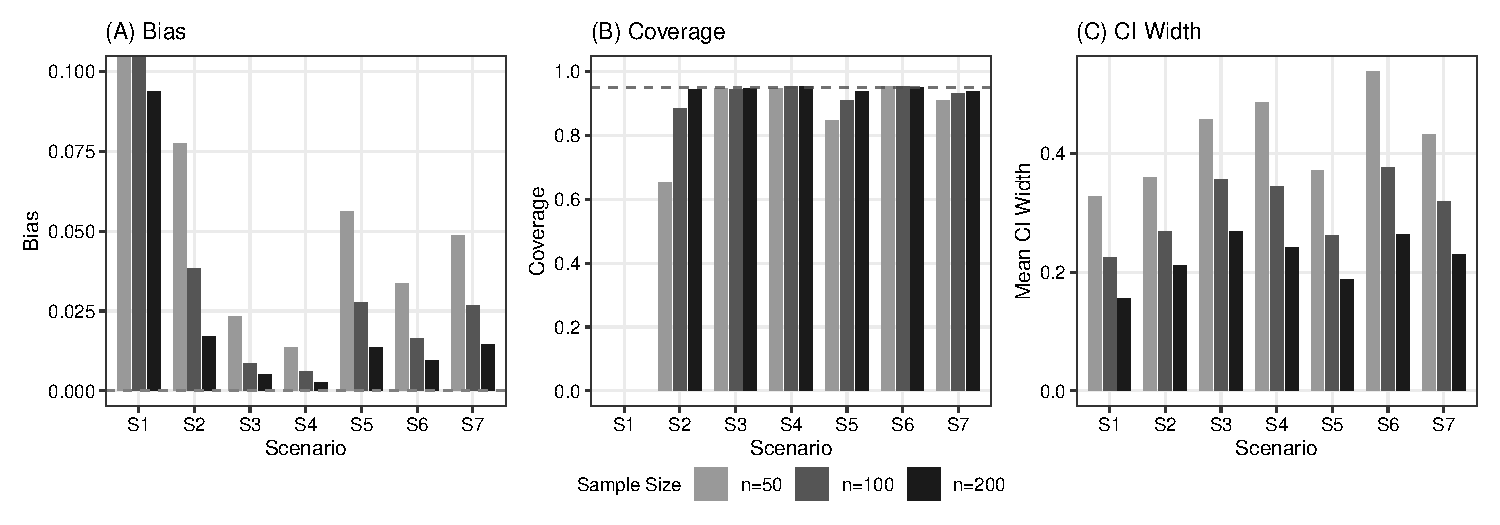
\includegraphics[width=\textwidth]{fig2_simulation_results.pdf}}
\caption{Estimation properties of $\hat{\rho} = \widehat{W}_1 / \widehat{\text{IQR}}_{\text{pooled}}$ across scenarios (S1--S7) and sample sizes ($n = 50, 100, 200$). Panel~(A): bias, with dashed horizontal line at zero. Panel~(B): coverage probability of 95\% percentile bootstrap CIs, with dashed line at the nominal 0.95 level; S1 coverage is structurally zero because the true value lies at the parameter space boundary (see Section~\ref{sec:sim_results}). Panel~(C): mean CI width in units of $\hat{\rho}$.\label{fig:simulation}}
\end{figure*}

Table~\ref{tab:coverage} presents coverage probabilities of the 95\% bootstrap confidence intervals. For scenarios with true $\rho$ above approximately 0.2, coverage was near-nominal at $n \geq 100$: S3 (0.945--0.946), S4 (0.954--0.955), S6 (0.951--0.954), and S7 (0.932--0.938). S4 (1.0$\sigma$ location shift) showed particularly stable coverage across all sample sizes, with no degradation at larger $n$, confirming satisfactory bootstrap performance even for large distributional differences. S5 (scale) showed moderate undercoverage at $n=50$ (0.847) that improved to near-nominal at $n=200$ (0.939). S2 (small location shift) showed undercoverage at $n=50$ (0.652) due to its near-boundary true value, improving to 0.943 at $n=200$.

Coverage for S1 (null) is shown as zero in Figure~\ref{fig:simulation}(B) because its true $\rho$ lies at the parameter space boundary. The non-negativity constraint produces persistent positive bias that prevents the finite-sample confidence interval from containing the true value of zero. This does not indicate estimator failure---the estimator is consistent---but rather that sample sizes well beyond 200 per region would be needed for reliable inference when the true distributional difference is negligible.

We also evaluated BCa (bias-corrected and accelerated) confidence intervals in preliminary experiments. BCa intervals showed consistently lower coverage than percentile intervals across all scenarios, particularly for near-boundary scenarios. The BCa correction overcorrects for $\hat{\rho}$ because the statistic is bounded below by zero, causing the acceleration parameter to distort the quantile adjustment. Based on these findings, we adopt percentile bootstrap as the primary inference method.

Monte Carlo standard errors for all reported coverage probabilities were below 0.005 at 10{,}000 replications, ensuring that observed differences across scenarios and sample sizes reflect genuine operating characteristic differences rather than simulation noise.

\begin{table}[ht]
\centering
\caption{Coverage probability of 95\% percentile bootstrap confidence intervals.\label{tab:coverage}}
\begin{tabular}{lccc}
\toprule
\textbf{Scenario} & $\boldsymbol{n=50}$ & $\boldsymbol{n=100}$ & $\boldsymbol{n=200}$ \\
\midrule
S2 (0.2$\sigma$) & 0.652 & 0.885 & 0.943 \\
S3 (0.5$\sigma$) & 0.946 & 0.945 & 0.946 \\
S4 (1.0$\sigma$) & 0.947 & 0.955 & 0.954 \\
S5 (Scale) & 0.847 & 0.910 & 0.939 \\
S6 (Skew) & 0.954 & 0.954 & 0.951 \\
S7 (Loc+Scale) & 0.911 & 0.932 & 0.938 \\
\bottomrule
\end{tabular}
\begin{tablenotes}
\item Coverage under S1 (Null) is shown as zero in Figure~\ref{fig:simulation}(B) but omitted from this table for brevity; the structural zero arises from the non-negativity constraint at the parameter space boundary.
\item For S4, coverage was near-nominal across all sample sizes (0.947--0.955), confirming satisfactory performance even for large distributional differences. The undercoverage for S2 at small sample sizes (0.652 at $n=50$) and S5 (0.847 at $n=50$) reflects boundary proximity effects that diminish with increasing $n$.
\end{tablenotes}
\end{table}

\subsubsection{Estimation Precision}

The mean CI width pattern across scenarios and sample sizes is shown in Figure~\ref{fig:simulation}(C). Table~\ref{tab:precision} presents the RMSE and mean CI width across scenarios. RMSE decreased consistently with increasing $n$, reaching values below 0.10 for all scenarios at $n = 200$. Mean CI width narrowed proportionally, with CIs at $n = 100$ typically spanning 0.22--0.38 in units of $\hat{\rho}$. In the clinical calibration framework, this CI width propagates to $\Delta_{\max}$ via $\Delta_{\max} = L_{\text{clinical}} \cdot W_1 = L_{\text{clinical}} \cdot \text{IQR}_{\text{pooled}} \cdot \rho$ (Supplement~A). For example, with $L_{\text{clinical}} = 0.01$/yr and $\text{IQR}_{\text{pooled}} = 17$ (values representative of age in the GUSTO-I application), a CI width of 0.27 in $\hat{\rho}$ corresponds to a $\Delta_{\max}$ CI width of $0.01 \times 17 \times 0.27 = 0.046$ (4.6\%pt)---a level of precision sufficient for meaningful clinical calibration.

\begin{table}[ht]
\centering
\caption{RMSE and mean CI width of $\hat{\rho}$ by scenario and sample size.\label{tab:precision}}
\begin{tabular}{lcccccc}
\toprule
& \multicolumn{3}{c}{\textbf{RMSE}} & \multicolumn{3}{c}{\textbf{Mean CI Width}} \\
\cmidrule(lr){2-4}\cmidrule(lr){5-7}
\textbf{Scenario} & $\boldsymbol{n=50}$ & $\boldsymbol{n=100}$ & $\boldsymbol{n=200}$ & $\boldsymbol{n=50}$ & $\boldsymbol{n=100}$ & $\boldsymbol{n=200}$ \\
\midrule
S1 (Null) & 0.20 & 0.14 & 0.10 & 0.33 & 0.22 & 0.16 \\
S2 (0.2$\sigma$) & 0.12 & 0.09 & 0.06 & 0.36 & 0.27 & 0.21 \\
S3 (0.5$\sigma$) & 0.13 & 0.10 & 0.07 & 0.46 & 0.36 & 0.27 \\
S4 (1.0$\sigma$) & 0.12 & 0.09 & 0.06 & 0.49 & 0.34 & 0.24 \\
S5 (Scale) & 0.11 & 0.07 & 0.05 & 0.37 & 0.26 & 0.19 \\
S6 (Skew) & 0.14 & 0.10 & 0.07 & 0.54 & 0.38 & 0.26 \\
S7 (Loc+Scale) & 0.12 & 0.09 & 0.06 & 0.43 & 0.32 & 0.23 \\
\bottomrule
\end{tabular}
\begin{tablenotes}
\item CI width is defined as mean of (upper $-$ lower) across 10{,}000 replications.
\end{tablenotes}
\end{table}

Under the null hypothesis (S1), the positive bias produces CIs that are shifted upward from zero. At $n = 50$, the mean estimate was 0.185 with mean CI width 0.33, and at $n = 200$, the mean estimate decreased to 0.094 with mean CI width 0.16. This bias is relevant for clinical calibration. When the true distributional difference is zero, the estimator will suggest a small positive $\Delta_{\max}$. Practitioners should be aware of this conservative tendency, particularly at smaller sample sizes.

\subsubsection{Comparison with Standardized Mean Difference}

Table~\ref{tab:smd} compares the sensitivity of $\hat{\rho}$ and SMD to different types of distributional differences. While both metrics respond to location shifts, SMD is insensitive to differences in variance and shape---the very types of distributional differences that may drive treatment effect heterogeneity through non-linear CATE functions.

\begin{table}[ht]
\centering
\caption{Sensitivity comparison: $\hat{\rho}$ versus SMD at $n=100$.\label{tab:smd}}
\begin{tabular}{lccc}
\toprule
\textbf{Scenario} & $\boldsymbol{\hat{\rho}}$ \textbf{(mean $\pm$ SD)} & \textbf{SMD (mean $\pm$ SD)} & \textbf{Implication} \\
\midrule
S3 (Location) & $0.367 \pm 0.097$ & $0.50 \pm 0.14$ & Both detect \\
S5 (Scale only) & $0.272 \pm 0.066$ & $0.00 \pm 0.14$ & Only $\hat{\rho}$ detects \\
S6 (Skew only) & $0.622 \pm 0.094$ & $0.00 \pm 0.14$ & Only $\hat{\rho}$ detects \\
\bottomrule
\end{tabular}
\begin{tablenotes}
\item SMD depends only on the difference in means, making it insensitive to differences in variance and skewness. $\hat{\rho}$ (and hence $\widehat{W}_1$) captures the full distributional difference. S6 is particularly informative because a large distributional difference ($\rho = 0.62$, corresponding to a substantial $W_1$ on the variable's natural scale) is entirely invisible to SMD.
\end{tablenotes}
\end{table}

In summary, the simulation study across seven scenarios demonstrates that the $\widehat{W}_1$ estimator (presented in the dimensionless form $\hat{\rho}$ for cross-scenario comparability) provides reliable estimation with the following properties at sample sizes typical in MRCT regional subgroups:
\begin{enumerate}[1.]
\item Bias: Less than 0.04 in $\hat{\rho}$ for most non-null scenarios at $n \geq 100$, with positive bias largest near the boundary (S1: 0.132 at $n = 100$) and negligible for scenarios with true $\rho$ above 0.2 (S3: 0.009, S4: 0.006 at $n = 100$).
\item Coverage: 0.88--0.96 at $n \geq 100$ for scenarios with true $\rho \geq 0.2$ (S3--S7); S6 (skew) and S7 (location + scale) achieved coverage between 0.91--0.95.
\item Precision: RMSE below 0.12 and CI width below 0.38 at $n \geq 100$.
\item Sensitivity: Captures location, scale, and skewness differences where SMD is limited to location only.
\end{enumerate}

Scenario S3 (0.5$\sigma$ location shift, true $\rho = 0.358$) exemplifies the operating characteristics at clinically relevant effect sizes. Bias was negligible ($+0.009$ at $n = 100$), coverage was nominal (0.945), and CI width (0.36) translated to a $\Delta_{\max}$ CI width of $0.01 \times 17 \times 0.36 = 0.061$ (6.1\%pt) when calibrated with $L_{\text{clinical}} = 0.01$/yr and $\text{IQR}_{\text{pooled}} = 17$ (age-scale parameters representative of the GUSTO-I application)---a level of precision sufficient for informed regulatory deliberation.

These estimation properties ensure that $\widehat{W}_1$, when combined with the clinical calibration framework of Section~\ref{sec:inference}, provides $\Delta_{\max}$ estimates of sufficient quality for regulatory deliberation. We recommend $n \geq 100$ per region for reliable estimation and inference.

%==============================================================================
\section{Application: Hypothetical Thrombolytic MRCT Using GUSTO-I Data}\label{sec:application}
%==============================================================================

We illustrate the per-EM Wasserstein-1 framework through a hypothetical scenario grounded in publicly available data from GUSTO-I, a large international trial in acute myocardial infarction (AMI). A sponsor is developing a novel thrombolytic agent (Drug~T) for AMI and is planning a Phase~3 MRCT across multiple regions. At the planning stage, the sponsor uses IPD from GUSTO-I ($N = 40{,}830$; 16 regions)\cite{gusto1993} to assess distributional similarity of candidate effect modifiers across regions and to identify suitable pooling partners for a designated anchor region. GUSTO-I was not designed as an MRCT and its regions are anonymized.

\subsection{Scenario Design and Effect Modifier Selection}\label{sec:app_scenario}

For this illustrative exercise, the sponsor identifies two candidate effect modifiers for Drug~T's treatment effect in AMI: age and systolic blood pressure (SBP). Drug~T is a novel agent. Its Phase~2 programme has suggested age and SBP as candidate effect modifiers on the basis of exploratory analyses and biological plausibility, but the precision of these analyses is insufficient for numerical estimation of $L_{\text{clinical}}$. At this planning stage the sponsor therefore has no quantitative prior on the clinical slope $L_{\text{clinical}}$ for either candidate effect modifier, and class-level indirect evidence is of limited value as a numerical substitute. For age, the Fibrinolytic Therapy Trialists' (FTT) collaborative meta-analysis of existing fibrinolytic agents\cite{ftt1994} concluded benefit is present irrespective of age and does not report a per-year CATE slope on the absolute mortality scale, so class transferability would not yield a defensible numerical prior for Drug~T. For SBP, no class-level quantitative estimate of clinical slope is available at all. We therefore treat $L_{\text{clinical}}$ as unknown a priori for both candidate effect modifiers, and apply the $L^*$ reverse-calculation pathway (equation~\ref{eq:lstar}) to both.

The sponsor selects Region~8 as the anchor region---representing, for instance, a regulatory market where local efficacy evidence is required but sample size is limited. Region~8 comprises $n = 2{,}916$ patients in GUSTO-I, with baseline characteristics summarized in Table~\ref{tab:gusto_r8}. The exercise of identifying Region~8's suitable pooling partners simulates the decision a sponsor would face when seeking regional efficacy assessment through pooling as described in ICH E17.\cite{iche17}

\begin{table}[ht]
\centering
\caption{Region~8 baseline characteristics (GUSTO-I).\label{tab:gusto_r8}}
\begin{tabular}{lcccc}
\toprule
\textbf{Candidate effect modifier} & \textbf{Mean} & \textbf{SD} & \textbf{Skewness} & \textbf{IQR\textsubscript{pooled}} \\
\midrule
Age (years) & 60.2 & 12.1 & $-0.17$ & 17--18 \\
SBP (mmHg) & 132.4 & 22.9 & 0.20 & 30--34 \\
\bottomrule
\end{tabular}
\begin{tablenotes}
\item $n = 2{,}916$. IQR\textsubscript{pooled} ranges reflect variation across the 15 partner-region pairs.
\end{tablenotes}
\end{table}

\subsection{Distributional Assessment: Per-EM W₁ Across 15 Partner Regions}\label{sec:app_nabcd}

We computed $\widehat{W}_1$ between Region~8 and each of the remaining 15 regions for both candidate effect modifiers, expressed in the original measurement units (years for age, mmHg for SBP), with percentile bootstrap 95\% confidence intervals ($B = 2{,}000$). Table~\ref{tab:gusto_nabcd} presents the results. Figure~\ref{fig:gusto_forest} displays these results as a forest plot with bootstrap CIs, with partners ordered by ascending $\widehat{W}_{1,\text{age}}$ to aid visual comparison.

\begin{table}[ht]
\centering
\caption{Per-EM Wasserstein-1 distance $\widehat{W}_1$ in original variable units (years for age, mmHg for SBP) with 95\% percentile bootstrap CIs for Region~8 versus each partner region (GUSTO-I), listed by region number.\label{tab:gusto_nabcd}}
\begin{tabular}{lrll}
\toprule
\textbf{Partner} & $n$ & $\boldsymbol{\widehat{W}_{1,\text{age}}}$ \textbf{(yr) [95\% CI]} & $\boldsymbol{\widehat{W}_{1,\text{SBP}}}$ \textbf{(mmHg) [95\% CI]} \\
\midrule
R1  & 2188 & 0.65 [0.51, 1.03] & 3.61 [2.68, 4.93] \\
R2  & 2952 & 2.15 [1.57, 2.76] & 0.95 [0.76, 1.82] \\
R3  & 2030 & 2.61 [1.96, 3.28] & 3.35 [2.32, 4.65] \\
R4  & 2876 & 0.56 [0.37, 1.16] & 2.60 [1.82, 3.75] \\
R5  & 1909 & 0.39 [0.35, 0.92] & 3.37 [2.32, 4.59] \\
R6  & 1585 & 0.91 [0.63, 1.39] & 3.37 [2.06, 4.77] \\
R7  & 3150 & 0.40 [0.30, 0.95] & 5.07 [4.03, 6.22] \\
R9  & 3123 & 0.59 [0.40, 1.12] & 6.80 [5.71, 8.01] \\
R10 & 1717 & 1.38 [0.79, 2.13] & 4.00 [2.88, 5.39] \\
R11 & 2491 & 1.27 [0.76, 1.91] & 6.44 [5.25, 7.71] \\
R12 & 4352 & 0.86 [0.47, 1.43] & 6.40 [5.39, 7.46] \\
R13 & 2297 & 1.15 [0.76, 1.74] & 2.40 [1.42, 3.72] \\
R14 & 3437 & 0.70 [0.42, 1.29] & 4.36 [3.41, 5.44] \\
R15 & 2576 & 0.61 [0.40, 1.25] & 4.72 [3.60, 5.94] \\
R16 & 1231 & 1.74 [1.16, 2.47] & 4.28 [3.06, 5.71] \\
\bottomrule
\end{tabular}
\begin{tablenotes}
\item Point estimates with 95\% percentile bootstrap CIs ($B = 2{,}000$, seed = 2026). Regions are listed by region number, and ordering carries no implicit ranking. Bootstrap CIs quantify estimation uncertainty. Narrow CIs lend greater confidence to individual $\widehat{W}_1$ values, while overlapping CIs indicate partners whose relative position is not sharply resolved by the data.
\end{tablenotes}
\end{table}

\begin{figure}[ht]
\centering
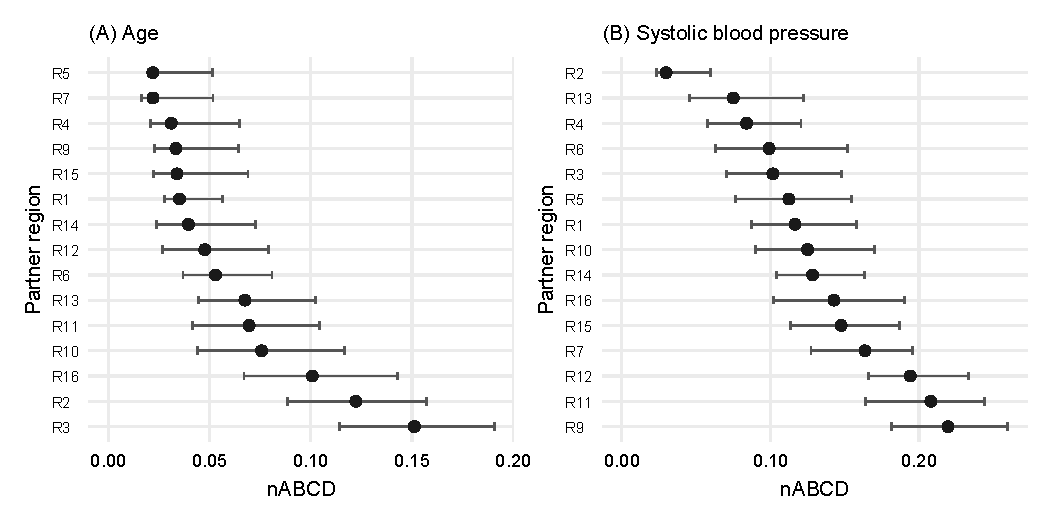
\includegraphics[width=0.8\textwidth]{fig3_gusto_r8_forest.pdf}
\caption{Forest plots of $\widehat{W}_1$ point estimates in original units (years for age, panel A; mmHg for SBP, panel B) with 95\% percentile bootstrap CIs. Partners are ordered by ascending $\widehat{W}_1$ within each panel; ordering and horizontal scale differ between panels.}
\label{fig:gusto_forest}
\end{figure}

The two candidate effect modifiers produce different patterns of distributional similarity. For age, partner-region $\widehat{W}_{1,\text{age}}$ point estimates span from 0.39 years (R5) at the low end to 2.61 years (R3) at the high end, with most partners below 1.5 years. For SBP, point estimates span from 0.95 mmHg (R2) to 6.80 mmHg (R9). Relative to their respective natural scales (age IQR \(\approx 17\)--18 years and SBP IQR \(\approx 30\)--34 mmHg in Region~8), the SBP differences are slightly larger in proportion than the age differences, and the ranking of partners by each candidate effect modifier differs accordingly.

Several partners fall in the middle of each ranking where uncertainty intervals overlap substantially. R16's $\widehat{W}_{1,\text{age}}$ ($1.74$ years) is the 13th-smallest value with 95\% CI $[1.16, 2.47]$ years, placing it in a region where its relative position is not sharply determined by the data---the CI spans the range covered by several partners with smaller point estimates. R6's $\widehat{W}_{1,\text{age}}$ ($0.91$ years) is the 9th-smallest value, while its $\widehat{W}_{1,\text{SBP}}$ of $3.37$ mmHg sits in the lower-middle of the SBP distribution with 95\% CI $[2.06, 4.77]$ mmHg, similarly spanning a broad region of the SBP ranking. These mid-rank cases illustrate the value of reporting bootstrap CIs alongside point estimates. The ranking itself is accompanied by an uncertainty interval that informs how confidently one partner can be placed above or below another.

An instructive contrast emerges between R2 and R9. R2 has the second-largest $\widehat{W}_{1,\text{age}}$ (2.15 years) but the smallest $\widehat{W}_{1,\text{SBP}}$ (0.95 mmHg), while R9 has the 4th-smallest $\widehat{W}_{1,\text{age}}$ (0.59 years) but the largest $\widehat{W}_{1,\text{SBP}}$ (6.80 mmHg). A ranking based on either candidate effect modifier alone would reach opposite conclusions about these two regions. This asymmetry underscores the necessity of evaluating all candidate effect modifiers jointly.

\subsection{Clinical Interpretation and Pooling Candidates}\label{sec:app_clinical}

We require an upper bound on the clinical slope $L_{\text{clinical}}$ for each candidate effect modifier; recall that $L_{\text{clinical}}$ governs how strongly treatment effect varies with the modifier. For thrombolysis in acute myocardial infarction, class-level meta-analytic evidence (GUSTO-I,\cite{gusto1993} FTT collaborative meta-analysis,\cite{ftt1994} and the GUSTO-I prognostic model\cite{lee1995}) supports a conservative upper bound of approximately 10\%pt per decade for age-related and 2\%pt per 10~mmHg for SBP-related treatment effect modification on 30-day mortality, exceeding the empirical prognostic gradients in Lee et al.\cite{lee1995} We adopt these as illustrative bounds: $L_{\text{age,UB}} = 1\times10^{-2}$ /yr and $L_{\text{SBP,UB}} = 2\times10^{-3}$ /mmHg.

For each partner region, we compare the region-specific $L^*$ value (Table~\ref{tab:gusto_lstar_joint}) with the corresponding plausible upper bound $L_{\text{UB}}$. A region is judged eligible for pooling on a given effect modifier if $L^* > L_{\text{UB}}$, meaning the clinical slope required for the observed distributional difference to produce $\Delta_{\text{clin}} = 1$\%pt exceeds the plausible bound. On age, the eligible partners are R1, R4, R5, R6, R7, R9, R12, R14, R15 (nine regions with $L^*_{\text{age}} > 0.01$). On SBP, the eligible partners are R1, R2, R3, R4, R5, R6, R10, R13, R14, R15, R16 (eleven regions with $L^*_{\text{SBP}} > 0.002$); R7 ($L^*_{\text{SBP}} = 0.0020 = L_{\text{SBP,UB}}$) is excluded.

\begin{table}[ht]
\centering
\caption{Clinical interpretation ($L^*$ at $\Delta_{\text{clin}} = 1$\%pt) and joint eligibility for all 15 partner regions, listed by region number. $L^*$ is the minimum clinical slope (per year for age, per mmHg for SBP) required for the observed distributional difference to produce a treatment effect difference of $1$\%pt on the absolute 30-day mortality scale. Eligibility is judged $L^* > L_{\text{UB}}$ with $L_{\text{age},\text{UB}} = 1\times10^{-2}$ /yr and $L_{\text{SBP},\text{UB}} = 2\times10^{-3}$ /mmHg.\label{tab:gusto_lstar_joint}}
\begin{tabular}{lrrrrccc}
\toprule
\textbf{Partner} & $\boldsymbol{\widehat{W}_{1,\text{age}}}$ \textbf{(yr)} & $\boldsymbol{\widehat{W}_{1,\text{SBP}}}$ \textbf{(mmHg)} & \textbf{$L^*$ age (/yr)} & \textbf{$L^*$ SBP (/mmHg)} & \textbf{Age elig.} & \textbf{SBP elig.} & \textbf{Joint} \\
\midrule
R1  & 0.65 & 3.61 & 0.0154 & 0.0028 & \checkmark & \checkmark & \checkmark \\
R2  & 2.15 & 0.95 & 0.0047 & 0.0105 & --- & \checkmark & --- \\
R3  & 2.61 & 3.35 & 0.0038 & 0.0030 & --- & \checkmark & --- \\
R4  & 0.56 & 2.60 & 0.0179 & 0.0038 & \checkmark & \checkmark & \checkmark \\
R5  & 0.39 & 3.37 & 0.0256 & 0.0030 & \checkmark & \checkmark & \checkmark \\
R6  & 0.91 & 3.37 & 0.0110 & 0.0030 & \checkmark & \checkmark & \checkmark \\
R7  & 0.40 & 5.07 & 0.0247 & 0.0020 & \checkmark & --- & --- \\
R9  & 0.59 & 6.80 & 0.0171 & 0.0015 & \checkmark & --- & --- \\
R10 & 1.38 & 4.00 & 0.0072 & 0.0025 & --- & \checkmark & --- \\
R11 & 1.27 & 6.44 & 0.0079 & 0.0016 & --- & --- & --- \\
R12 & 0.86 & 6.40 & 0.0116 & 0.0016 & \checkmark & --- & --- \\
R13 & 1.15 & 2.40 & 0.0087 & 0.0042 & --- & \checkmark & --- \\
R14 & 0.70 & 4.36 & 0.0143 & 0.0023 & \checkmark & \checkmark & \checkmark \\
R15 & 0.61 & 4.72 & 0.0164 & 0.0021 & \checkmark & \checkmark & \checkmark \\
R16 & 1.74 & 4.28 & 0.0057 & 0.0023 & --- & \checkmark & --- \\
\bottomrule
\end{tabular}
\begin{tablenotes}
\item Regions are listed by region number, and ordering carries no implicit ranking. \checkmark{} indicates eligibility ($L^* > L_{\text{UB}}$); --- indicates ineligibility.
\end{tablenotes}
\end{table}

A region is jointly eligible if it satisfies the criterion on both candidate effect modifiers, since pooling requires distributional compatibility across all evaluated modifiers. Six regions meet this AND condition: R1, R4, R5, R6, R14, R15. The remaining nine partners fail on at least one effect modifier---for example, R2 fails on age ($L^*_{\text{age}} = 0.0047$), R9 fails on SBP ($L^*_{\text{SBP}} = 0.0015$)---and are not recommended for pooling under these clinical assumptions.

Among the jointly eligible partners, R4 emerges as the leading single-pool candidate. R4 ranks 3rd-lowest on age ($\widehat{W}_{1,\text{age}} = 0.56$ years) and 3rd-lowest on SBP ($\widehat{W}_{1,\text{SBP}} = 2.60$ mmHg), balanced across both modifiers. R5 has the lowest age value ($\widehat{W}_{1,\text{age}} = 0.39$ years) but a mid-rank SBP value ($\widehat{W}_{1,\text{SBP}} = 3.37$ mmHg), an asymmetric profile. The framework supplies the quantitative inputs ($\widehat{W}_1$ with bootstrap CIs in Table~\ref{tab:gusto_nabcd}, partner-specific $L^*$ in Table~\ref{tab:gusto_lstar_joint}, and joint eligibility under the assumed bounds) to support sponsor judgment in consultation with clinical and regulatory advisors. Note that the GUSTO-I data were collected during 1990--1993; the application here serves as methodological illustration using publicly available IPD, not as an endorsement of these specific distributions for contemporary thrombolytic-trial planning.

%==============================================================================
\section{Discussion}\label{sec:discussion}
%==============================================================================

This paper addresses three methodological gaps identified in Section~\ref{sec:existing}, demonstrating that nABCD: (i) captures scale and skewness differences in regional effect modifier distributions that are invisible to standardized mean differences, as confirmed by simulation scenarios with location-preserving variance and shape contrasts (S5, S6); (ii) translates distributional distance into a clinically interpretable scale via the heterogeneity bound \(\Delta_{\max}\) (equation~\ref{eq:delta_max}), providing a theoretical link to regional treatment effect heterogeneity that is absent in empirical-distribution-function tests such as the Kolmogorov--Smirnov statistic; and (iii) admits reliable percentile bootstrap inference for non-negligible distributional differences at moderate sample sizes (\(n \geq 100\) per region, coverage 0.88--0.96 across S2--S7), while exhibiting characterized boundary behavior near the null that delimits the operational range of inference.

These methodological findings carry two interpretive implications for pooling decisions, illustrated by the GUSTO-I application as a worked example of the framework's operation rather than a substantive epidemiological claim. First, when multiple candidate effect modifiers are under consideration, all candidates must be evaluated jointly. A partner ranked similar on one effect modifier may not be similar on another, as exemplified by the contrast between R2 and R9. Restricting evaluation to a subset of candidates risks selecting partners whose distributional differences on the omitted modifiers would later compromise consistency. Second, partner selection cannot rest on nABCD ranking alone. The required CATE sensitivity $L^*$ that would translate a given nABCD into a clinically meaningful $\Delta_{\max}$ varies markedly across partners and across candidate effect modifiers, so the same nABCD value carries different clinical weight depending on the partner-specific distributional differences. In the GUSTO-I example, six partners (R1, R4, R5, R6, R14, R15) emerged as jointly eligible because their $L^*$ values exceeded the plausible bounds reviewed in Section~\ref{sec:application}; R4 stood out as the leading single-pool candidate due to its balanced ranking on both modifiers. Pooling judgments therefore require both distributional ranking and clinical calibration, applied across the full set of candidate effect modifiers.

Section~\ref{sec:existing} identified three gaps in existing distributional measures. SMD captures only location. The KS statistic and related EDF tests lack a clinically interpretable scale and a theoretical link to treatment effect heterogeneity. KL divergence is asymmetric, can diverge under non-overlapping support, and requires density estimation impractical at small regional samples. nABCD addresses all three. Where SMD captures only the mean, our simulation confirmed that scale (S5) and skewness (S6) differences produced near-zero SMD yet non-negligible nABCD. Where the KS statistic offers no clinical-scale translation, the IQR normalization and the heterogeneity bound (equation~\ref{eq:delta_max}) translate distributional distance into clinically meaningful units. Where KL divergence is asymmetric and prone to instability under limited sample overlap, nABCD is symmetric, finite for any pair of empirical distributions, and computable directly from CDFs without density estimation, while remaining amenable to bootstrap inference.

Two principal strengths follow from the dual-pathway clinical calibration. First, the framework adapts to where the trial sits on the spectrum of CATE sensitivity evidence, rather than imposing a fixed nABCD cutoff. At the MRCT planning stage, where $L$ is typically unavailable for novel agents, the $L^*$ reverse-calculation (equation~\ref{eq:lstar}) serves as the primary calibration tool. When $L$ is available from prior evidence, the $\Delta_{\max}$ pathway (equation~\ref{eq:delta_max}) provides a complementary calibration on the clinical scale. Second, nABCD's value as a distributional measure, capturing scale and skewness differences invisible to SMD, holds regardless of whether $L$ is available. Clinical calibration enhances but does not replace this distributional assessment.

For practice, we recommend computing nABCD with bootstrap CIs at moderate sample sizes (Section~\ref{sec:simulation}) for every candidate effect modifier across region pairs, translating each into $\Delta_{\max}$ (when $L$ is estimable) or $L^*$ at pre-specified $\Delta_{\text{clin}}$ values (when $L$ is unknown), and reporting these alongside clinically relevant benchmarks (overall treatment effect, non-inferiority margin) to support deliberation rather than binary decisions. When multiple candidate effect modifiers are evaluated, sponsors may adopt a conservative approach based on the maximum $\Delta_{\max}$ (or smallest $L^*$) across all effect modifiers and region pairs, or a totality-of-evidence approach in which the full collection---together with bootstrap uncertainty and the reliability of each $L$ estimate---informs holistic judgment. The choice depends on regulatory context.

For policy, the framework's compatibility with diverse data sources is a distinctive practical advantage. Because nABCD requires only baseline effect modifier distributions, regional data can be assembled from prior trials, registries, electronic health records, or other real-world evidence (RWE) sources---an increasingly relevant capability as regulatory agencies promote RWE use in drug development (ICH E6(R3)). The framework is particularly relevant for regulatory submissions requiring regional subpopulation consistency.\cite{matsushima2024,song2025} Matsushima et al.'s\cite{matsushima2024} PMDA workshop documented how regional imbalance in CRP-positive/MRI-negative status caused apparent inconsistency in the secukinumab MRCT, underscoring the practical consequences when effect modifier distributional differences are not assessed prospectively.

nABCD is one input within a holistic regulatory evaluation; biological plausibility, clinical relevance, and benefit--risk balance extend beyond what any single distributional measure can quantify.\cite{iche17,matsushima2024} The framework has further limitations. It treats continuous effect modifiers marginally, leaving categorical and multivariate extensions for future work. As a non-negative function of the Wasserstein distance, nABCD exhibits positive bias and zero bootstrap coverage when the true value lies at or near zero (S1; Section~\ref{sec:sim_results}),\cite{andrews2000} so we recommend $n \geq 100$ per region and cautious interpretation of estimates near the null. Clinical calibration depends on the CATE sensitivity $L$, which may be unavailable for novel agents (handled by the $L^*$ pathway) or transferred from prior evidence (a clinical assumption); the framework supplies quantitative inputs but prescribes no cutoffs. Finally, as with any covariate-based approach, unmeasured effect modifiers may contribute to heterogeneity beyond what the index captures.

Beyond the scope and methodological extensions noted above, two further directions warrant investigation. The upstream identification of which baseline characteristics constitute relevant effect modifiers is itself a non-trivial problem deserving dedicated treatment. Bias-correction methods tailored to the boundary behavior of nABCD at small samples could extend the operational range of inference. The principal contribution of this paper is to supply a quantitative tool where one was previously absent. nABCD, combined with bootstrap confidence intervals and clinical calibration via $\Delta_{\max}$ or $L^*$, transforms the previously qualitative judgment of ``similar enough'' into a reproducible, quantitative basis for sponsor judgment, filling the methodological gap left by ICH E17 and enabling evidence-based, clinically grounded pooling decisions.

%==============================================================================
% Back matter
%==============================================================================

\bmsection*{Author contributions}

[Author 1] conceived the research question and led the project. [Author 2] developed the mathematical framework and conducted the simulation study. [Author 3] contributed to the application example and manuscript preparation. All authors reviewed and approved the final manuscript.

\bmsection*{Acknowledgments}

The authors thank [colleagues] for helpful discussions on ICH E17 implementation.

\bmsection*{Financial disclosure}

None reported.

\bmsection*{Conflict of interest}

The authors declare no potential conflict of interests.

\bmsection*{Data availability statement}

R code for computing nABCD and reproducing the simulation study is available at [repository URL]. GUSTO-I individual patient data are available from the original investigators subject to applicable data sharing policies; the dataset is described in the original publication.\cite{gusto1993}

\bibliography{per_em_W1_wiley}

\bmsection*{Supporting information}

Additional supporting information may be found in the online version of the article at the publisher's website. Supporting materials include: complete R code for nABCD computation, simulation scripts, and additional figures for realistic clinical scenarios.

%==============================================================================
\appendix
%==============================================================================

\bmsection{Proofs and Mathematical Details\label{app:proofs}}

\bmsubsection{Proof of Proposition~\ref{prop:nonnegativity}\label{app:proof1}}

Non-negativity follows directly from the non-negativity of the Wasserstein-1 distance: $W_1(F_1, F_2) = \int |F_1(x) - F_2(x)| \, dx \geq 0$. Since $\text{IQR}_{\text{pooled}} > 0$ for non-degenerate distributions, the ratio $\text{nABCD} = W_1 / \text{IQR}_{\text{pooled}} \geq 0$.

For the identity of indiscernibles, we show both directions. If $F_1 = F_2$, then $|F_1(x) - F_2(x)| = 0$ for all $x$, so $W_1(F_1, F_2) = 0$ and hence $\text{nABCD} = 0$. Conversely, if $\text{nABCD} = 0$, then $W_1(F_1, F_2) = \int |F_1(x) - F_2(x)| \, dx = 0$. Since $|F_1(x) - F_2(x)| \geq 0$ and is right-continuous, $\int |F_1(x) - F_2(x)| \, dx = 0$ implies $F_1(x) = F_2(x)$ almost everywhere, and by right-continuity of CDFs, $F_1 = F_2$ everywhere.

\bmsubsection{Asymptotic Properties\label{app:asymptotic}}

Under standard regularity conditions, the empirical Wasserstein-1 distance $W_1(\hat{F}_1, \hat{F}_2)$ is a consistent estimator of $W_1(F_1, F_2)$.\cite{delbarrio1999} Combined with the consistency of the empirical IQR, $\hnABCD$ is a consistent estimator of $\text{nABCD}(F_1, F_2)$.

In one dimension, the empirical $W_1$ distance converges at rate $O(n^{-1/2})$ without logarithmic correction.\cite{delbarrio1999} For two-sample estimation with $F_1 \neq F_2$ and finite second moments, $\sqrt{n}(W_1(\hat{F}_{1,n_1}, \hat{F}_{2,n_2}) - W_1(F_1, F_2))$ converges in distribution to a mean-zero Gaussian, where $n = n_1 + n_2$ with $n_1/n \to \lambda \in (0,1)$. Since the empirical IQR also converges at rate $O(n^{-1/2})$ under standard density conditions, the delta method applied to the ratio $g(w, q) = w/q$ yields asymptotic normality of $\hnABCD$:
\begin{equation}
\sqrt{n}\bigl(\hnABCD - \text{nABCD}(F_1, F_2)\bigr) \xrightarrow{d} N(0,\, \sigma^2_{\text{nABCD}}),
\label{eq:asymptotic_normality}
\end{equation}
where $\sigma^2_{\text{nABCD}}$ depends on the asymptotic variances and covariance of the $W_1$ and IQR estimators. This result requires $\text{nABCD} > 0$ (i.e., $F_1 \neq F_2$). At the boundary $F_1 = F_2$, the parameter lies on the edge of the parameter space and standard asymptotics do not apply (see Section~\ref{sec:discussion}).

The bootstrap provides valid inference for the Wasserstein distance under mild conditions.\cite{sommerfeld2018} The percentile bootstrap confidence interval achieves asymptotically correct coverage for non-degenerate distributions.

\bmsection{R Code for nABCD Computation\label{app:rcode}}

\begin{lstlisting}[caption={R function for computing nABCD with bootstrap confidence intervals.},label=lst:nabcd,basicstyle=\fontsize{8}{10}\selectfont\ttfamily]
compute_nABCD <- function(x1, x2) {
  pooled <- c(x1, x2)
  iqr_pooled <- IQR(pooled)
  if (iqr_pooled == 0) return(NA)
  all_vals <- sort(unique(pooled))
  F1 <- ecdf(x1); F2 <- ecdf(x2)
  w1 <- sum(diff(all_vals) *
    abs(F1(all_vals[-length(all_vals)]) -
        F2(all_vals[-length(all_vals)])))
  w1 / iqr_pooled
}

nABCD_bootstrap <- function(x1, x2,
    B = 2000, conf = 0.95) {
  obs <- compute_nABCD(x1, x2)
  boot_vals <- replicate(B, {
    b1 <- sample(x1, replace = TRUE)
    b2 <- sample(x2, replace = TRUE)
    compute_nABCD(b1, b2)
  })
  alpha <- 1 - conf
  ci <- quantile(boot_vals,
    c(alpha/2, 1 - alpha/2), na.rm = TRUE)
  list(estimate = obs,
       ci_lower = ci[1], ci_upper = ci[2])
}
\end{lstlisting}

\end{document}
